% !TeX encoding = UTF-8
% !TeX spellcheck = en_US
\section{Linux kernel configuration/build}
\IEEEPARstart{T}he Linux kernel is developed by programmers from all around the world 
and can be obtained at \cite{Kernel_1}.
A mirrored version of the Linux kernel can be found on Github \cite{Kernel_2}.
The kernel is developed, compiled and installed by using Unix-like tools.
The main documentation is provided as plain text files while the kernel itself is programmed 
in the C programming language. Although the kernel itself is developed in C and Assembler,
some of the included helper tools are written in C++, in Bash shell scripts, or even in Python 
(e.g., see {\it tools/perf/python/}) or in Perl (e.g., see {\it tools/perf/perl}).
The Linux kernel also uses its own ecosystem of ``programming languages'' for configuration and 
building of the binary objects which are somehow ``domain-specific languages'', 
which have historically grown over time. 
\begin{figure*}[ht]
  \centering
  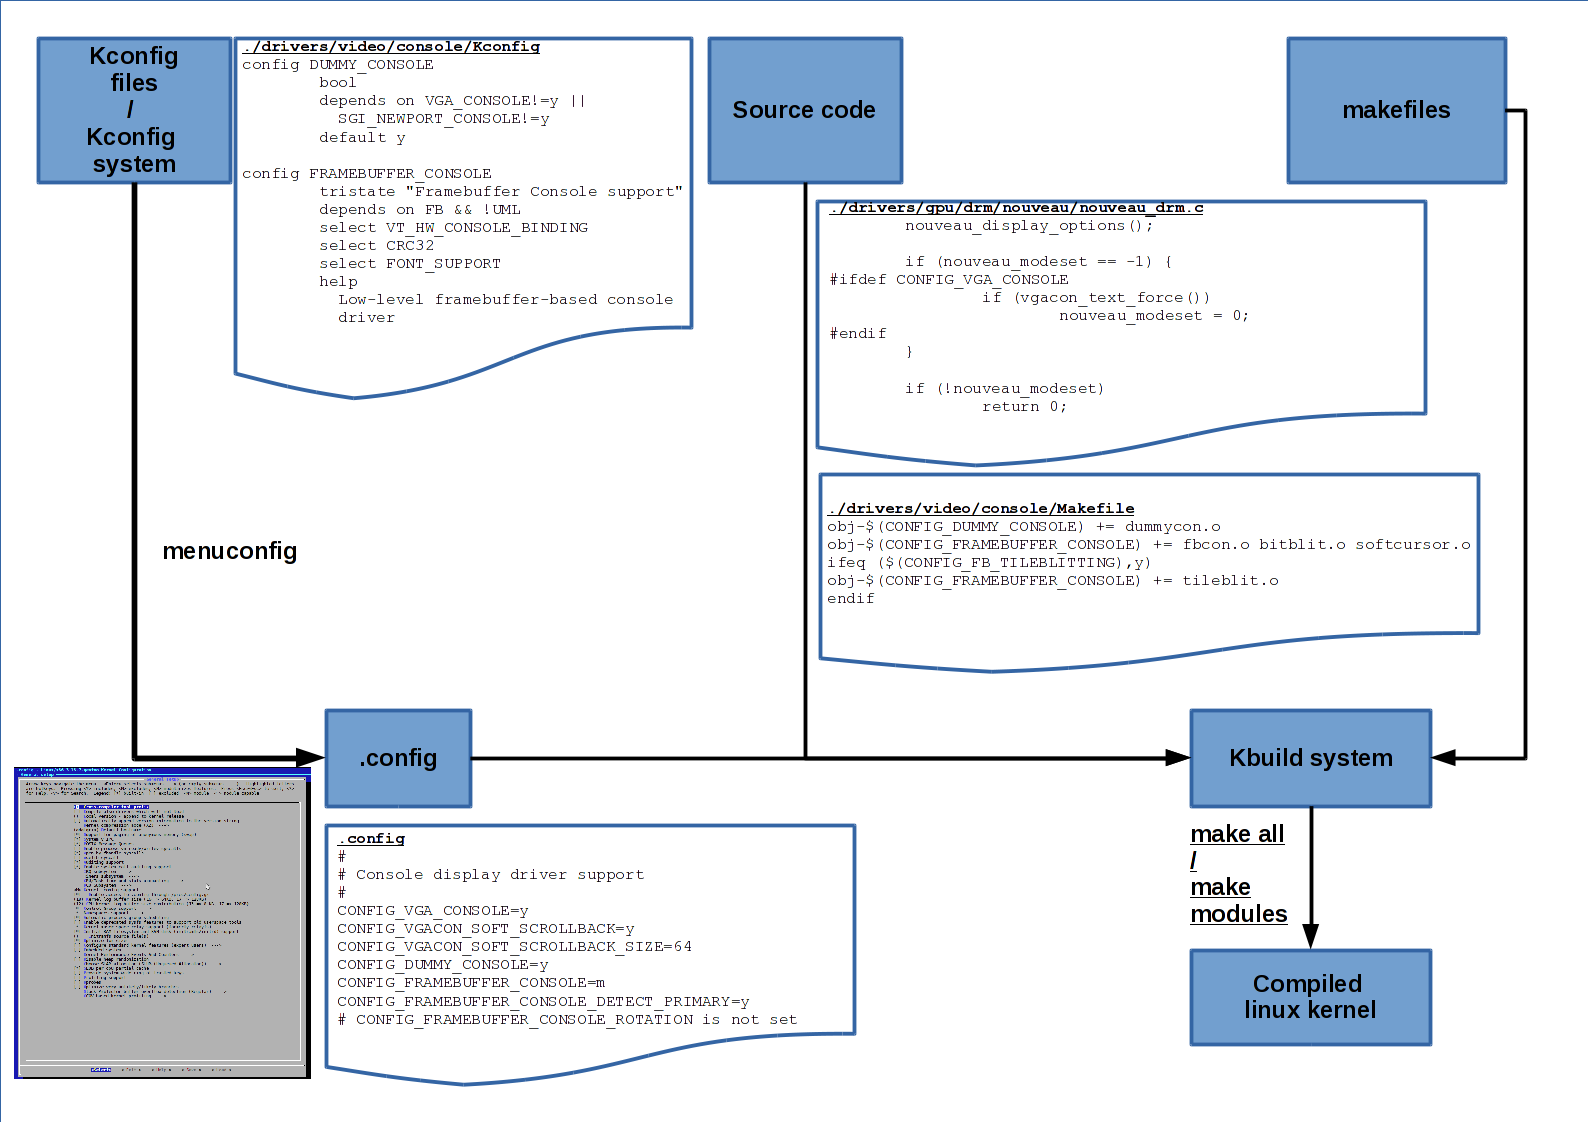
\includegraphics[scale=0.4]{images/overview}
  \caption{Overview over the Linux kernel configuration and build process}
  \label{fig:overview}
\end{figure*}

The picture \ref{fig:overview} shows an overview of the dependencies between the different ``DSLs''.
An overview of the kernel compilation and building can also be found at 
\cite{Kernel_3}
\FloatBarrier

\subsection{.config}

First, the Kconfig system specifies which features depend on each other or can not be combined together. 
Therefore, kconfig serves as some kind of non-formalized feature model.
Here is an example:
\lstinputlisting[frame=single,extendedchars=true,label=Kconfig,caption={./drivers/video/console/Kconfig},
  breaklines=true,]{code/driversVideoConsoleKconfig.txt}

A detailed description of the kconfig system can be found at \cite{Kernel_4} 
\\ \ \\
The variability model of the Linux kernel is, e.g., described in She et al. 
``The Variability Model of The Linux Kernel''\cite{she2010variability},
in Sincero et al. ``The Linux Kernel Configurator as a Feature Modeling Tool''\cite{sincero2008linux}
and in Tartler et al. ``Dead or alive: finding zombie features in the linux kernel
''\cite{tartler2009dead}.
Although these papers describe older kernel versions their main conclusions are still valid.

\subsection{Generating a .config file}

The users can then use one of the configuration tools which get delivered with the Linux kernel,
e.g. {\it make oldconfig} when you already have a running kernel and you want to only 
update to a new kernel version or 
{\it make menuconfig}, etc.
These applications use the kconfig files as input to determine which additional features 
must be selected or hide options which are not available due to conflicts.
The configuration is then saved into a {\it .config} file at the root directory of the 
Linux kernel source code.

The following text listing is an example for such a generated configuration file:
\lstinputlisting[frame=single,extendedchars=true,label=DotConfig,caption={.config file snippet},
  breaklines=true,]{code/dotConfig.txt}
\FloatBarrier

The following screenshot in figure \ref{fig:menuconfig} 
shows the {\it menuconfig} program, 
a graphical configuration tool which can be used on the terminal:
\begin{figure*}[ht]
  \centering
  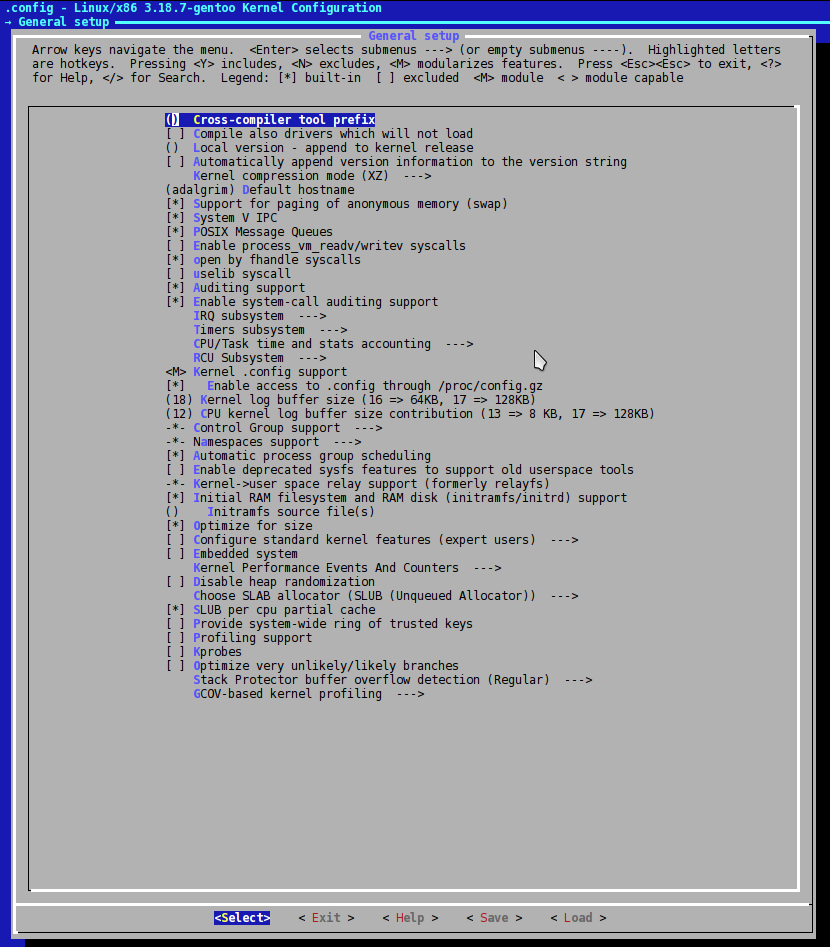
\includegraphics[scale=0.5]{images/menuconfig}
  \caption{Configuring the kernel with menuconfig, e.g., over a ssh connection}
  \label{fig:menuconfig}
\end{figure*}
\FloatBarrier

\subsection{Kbuild system}
Whenever the kernel, its modules or any initramfs should be built the kbuild system is invoked. 
Some valid targets for building are
\begin{itemize}
 \item make all
 \item make kernel
 \item make modules
 \item make vmlinux
 \item make initramfs
\end{itemize}

The makefile in the root directory of the linux source code then invokes the kbuild which 
generates / collects all necessary makefiles and processes them step-wise. 
Most of them just contain plain GNU make instructions but some contain additional bash script magic. 

An example kbuild makefile is the following:
\lstinputlisting[frame=single,extendedchars=true,label=Makefile,caption={Snippet from ./drivers/video/console/Makefile},
  breaklines=true,]{code/MakeFile.txt}
  
The commands in the makefile then instruct the C compiler which source files to compile and 
which command line options to use. The selected features of the {\it .config} file are 
provided as pre-processor macro definitions. But also include directories are enlisted. 

The following source snippet shows how the macro definitions are used in the C source code:
\lstinputlisting[frame=single,extendedchars=true,label=CSourceFile,caption={Snippet from ./drivers/gpu/drm/nouveau/nouveau\_drm.c},
  breaklines=true,]{code/CSourceFile.txt}
The results of the compilation are binary object files which can be installed to 
{\it /boot} and/or {\it /lib/modules/$<$linux-version$>$} with {\it make install}. 

More information about kbuild itself can be found at \cite{Kernel_5}
and
\cite{Kernel_6}
